\documentclass{beamer}
    \usetheme{Boadilla}
\usepackage{polyglossia}
    \setmainlanguage{german}
\usepackage{fontspec}
    \setsansfont{Linux Biolinum O}
\usepackage{graphicx}
\usepackage{xcolor}
\usepackage{listings}
    \lstset{language=bash,
	basicstyle=\footnotesize\ttfamily\tiny,
	breaklines=true,
	framextopmargin=50pt,
	frame=bottomline,
	backgroundcolor=\color{white!86!black},
	commentstyle=\color{blue},
	keywordstyle=\color{red},
	stringstyle=\color{orange!80!black}}
\usepackage{amsmath}
\usepackage{amssymb}
\usepackage{siunitx}
\usepackage{booktabs}
\usepackage{float}
\usepackage{tabularx}
\usepackage{caption}
\usepackage{subfig}
\usepackage{tikz}
\usepackage{hyperref}
     \hypersetup{
     colorlinks=true,
     linkcolor=black,
     filecolor=magenta}

\title{\texorpdfstring{\color{blue!50!black}\textbf{Status report - Wednesday, July 09th}}{}}
\subtitle{Preview and Cosmic Analysis}
\author{Maurice Donner}
\date{09. July 2020}

\begin{document}

\maketitle

\begin{frame}{Preview of Presentation for July 21st}

    \begin{minipage}{.4\textwidth}
	pdf can be found on indico \( \rightarrow \) 
    \end{minipage}
    \begin{minipage}{.59\textwidth}
	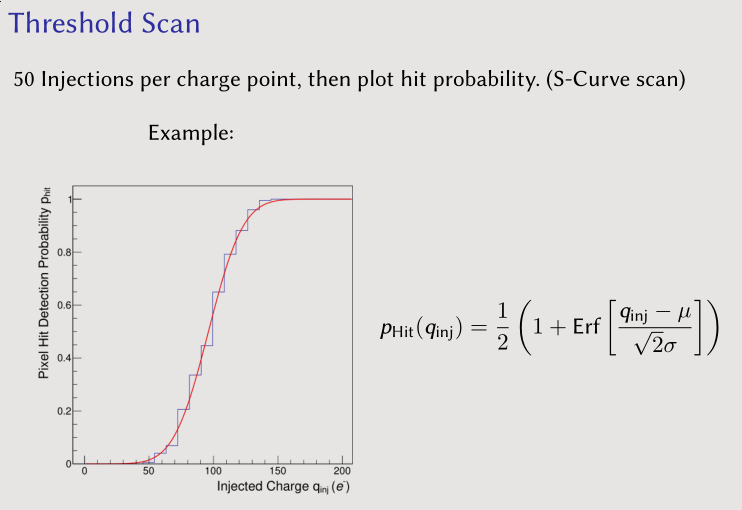
\includegraphics[width=\textwidth]{Preview.png}
    \end{minipage}
\end{frame}

\begin{frame}{Cosmic Analysis}
    \LARGE Problems \normalsize \\
    \begin{itemize}
	\item (so far) unable to calculate residuals in Corry
	\item "Good" tracks spread out over 1.5 TB of raw data \\
	    \( \rightarrow \) Using Corry for tracking very difficult (not able
	    to merge all data)
    \end{itemize}
    \pause
    \LARGE Workaround: \normalsize 
    Writing an Event organizer in python\\[.5cm]
    \centering
    \begin{tikzpicture}[font=\footnotesize, level 2/.style={sibling distance= .6cm}]
	\node {Hit\_Data}
	child { node { plane 1 } 
	    child { node { [X] } }
	    child { node { [Y] } }}
	child { node { plane 2 } 
	    child { node { [X] } }
	    child { node { [Y] } }}
	child { node { plane 3 } 
	    child { node { [X] } }
	    child { node { [Y] } }}
	child { node { plane 4 } 
	    child { node { [X] } }
	    child { node { [Y] } }}
	child { node { plane 5 } 
	    child { node { [X] } }
	    child { node { [Y] } }}
	child { node { plane 6 } 
	    child { node { [X] } }
	    child { node { [Y] } }}
	child { node { plane 7 } 
	    child { node { [X] } }
	    child { node { [Y] } }};
	\end{tikzpicture}
\end{frame}

\begin{frame}[fragile]{Cosmic Analysis}
    Feed it with DESY Testbeam Data, to calculate the average offset of the planes:
\begin{lstlisting}
Plane 1 position: X 13.74 Y -36.65
Plane 2 position: X 25.4 Y 16.19
Plane 3 position: X 30.15 Y 21.23
Plane 4 position: X 20.29 Y 20.06
Plane 5 position: X 20.65 Y -52.77
Plane 6 position: X -22.33 Y -41.59
\end{lstlisting}
\pause
\centering
\begin{minipage}{.13\textwidth}
    \tiny yes they're ugly, will produce some nicer plots soon!
\end{minipage}
\begin{minipage}{.30\textwidth}
    \centering
    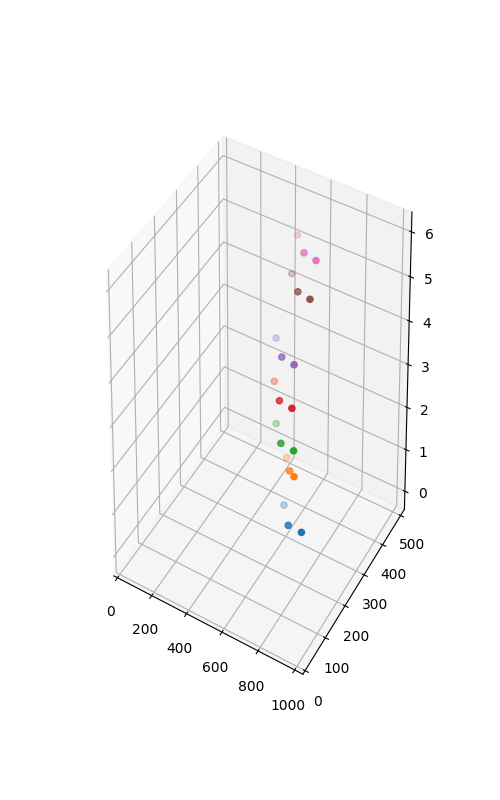
\includegraphics[trim=0 50 0 100,clip,width=\textwidth]{DESY_Before.png}
\end{minipage}
\begin{minipage}{.1\textwidth}
    \centering
    \( \rightarrow \)
\end{minipage}
\begin{minipage}{.30\textwidth}
    \centering
    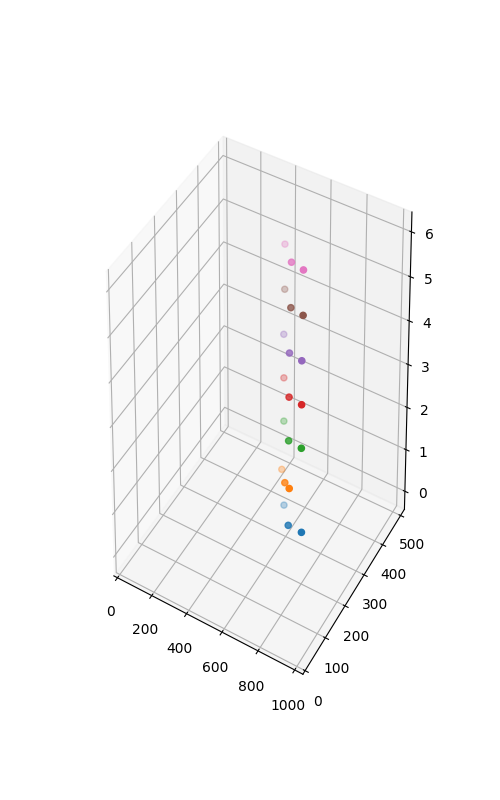
\includegraphics[trim=0 50 0 100,clip,width=\textwidth]{DESY_After.png}
\end{minipage}
\end{frame}

\begin{frame}{Cosmic Analysis}
    Some actual cosmics: (Before Alignment)
    \begin{figure}[H]
	\centering
	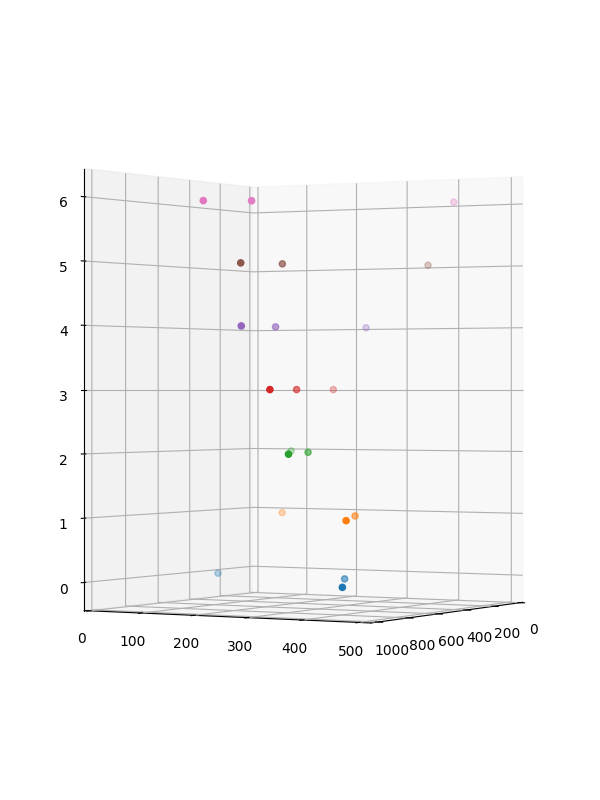
\includegraphics[trim=0 50 0 100,clip,width=.7\textwidth]{Before.png}
    \end{figure}
\end{frame}
\begin{frame}{Cosmic Analysis}
    Some actual cosmics: (After Alignment)
    \begin{figure}[H]
	\centering
	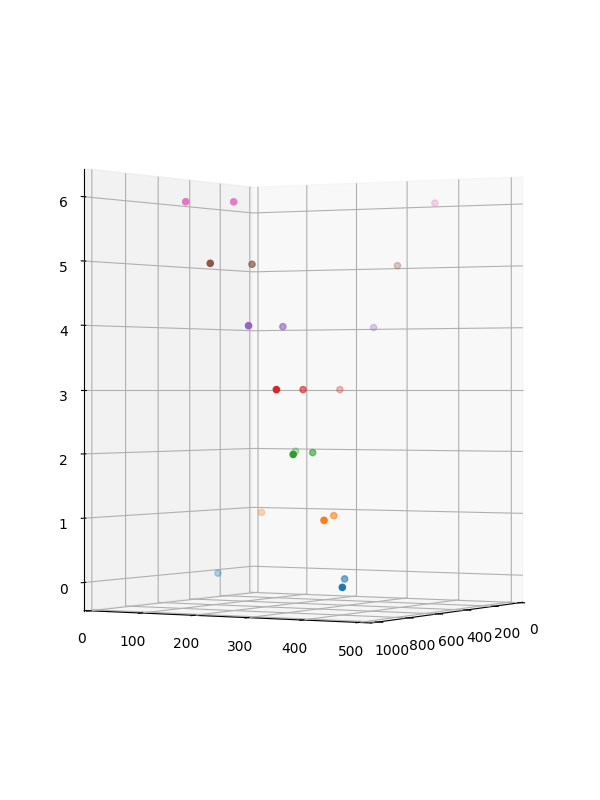
\includegraphics[trim=0 50 0 100,clip,width=.7\textwidth]{After.png}
    \end{figure}
\end{frame}

\begin{frame}{Outlook}
    Next possible steps:
    \begin{itemize}
	\item Further improge alignment by adding rotation \pause
	\item fitting straight tracks through the data and calculate residuals \pause
	\item Do some actual tracking and alignment with Cosmics \pause
	\item Produce some nicer Plots ;) \pause
    \end{itemize}
\end{frame}

\end{document}
